
\documentclass[10pt,a4paper]{article}
 
\usepackage[utf8x]{inputenc}
\usepackage[norsk]{babel}
\usepackage[T1]{fontenc,url}
\usepackage[hang,small,bf]{caption}
\usepackage{relsize}
\usepackage{setspace}
\usepackage{parskip}
\usepackage{lmodern}
\usepackage{microtype}
\usepackage{verbatim}
\usepackage{amsmath, amssymb, amsthm}
\usepackage{mathtools}
\usepackage{tikz}
\usepackage{physics}
\usepackage{algorithm}
\usepackage{algpseudocode}
\usepackage{listings}
\usepackage{enumerate}
\usepackage{graphicx}
\usepackage{float}
\usepackage{hyperref}
\usepackage{varioref}
\usepackage{siunitx}
\usepackage{todonotes}
\usepackage{color}
\usepackage[margin=3cm]{geometry}
\labelformat{equation}{ligning~(#1)}
 
\renewcommand{\exp}{\mathrm{e}^}
\newcommand{\halflife}{t_{\frac{1}{2}}}
\newcommand{\half}{\frac{1}{2}}
\newcommand{\planck}{$h = \SI{6.626e-34}{J.s}$}
 
\definecolor{light_green}{rgb}{0, 0.6, 0}
\definecolor{light_grey}{rgb}{0.5, 0.5, 0.5}
\definecolor{magenta}{rgb}{0.7, 0, 0.5}
 
 
\lstdefinestyle{py}{
    language = python,
    frame = single,
    showstringspaces = false,
    basicstyle = \small\ttfamily,
    breaklines = true,
    commentstyle = \color{light_grey},
    keywordstyle = \color{magenta},
    stringstyle = \color{light_green},
}
 
\begin{document}
\section*{Oppgave 3.1 - Radioaktiv funksjon}
\addcontentsline{toc}{section}{Oppgave 3.1 - Radioaktiv funksjon - \texttt{radioactive\_function.py}}
Implementer formelen for radioaktiv nedbrytning fra oppgave 1.3 som en funksjon \texttt{N(N0, tau, t)}.
 
Skriv en test-funksjon som bruker parametrene fra oppgave 1.3a, $N_0 = \SI{4.5}{kg}$, $\tau=\SI{1760}{s}$, $t=\SI{600}{s}$, og sjekk gjerne at svaret blir \SI{3.2}{kg} (som var resultatet fra 1.3a) innenfor en toleranse.
 
Ikke sett toleransen mindre enn $10^{-4}$, ettersom $3.2$ ikke er helt nøyaktig.
 
Filnavn: \texttt{radioactive\_function.py}
 
 
 
 

\section*{Oppgave 3.2 - Kvantefunksjon}
\addcontentsline{toc}{section}{Oppgave 3.2 - Kvantefunksjon - \texttt{quantum\_function.py}}
I oppgave 2.5 så vi at partikler fanget i en boks på størrelse $L$ bare kan ha energier
\[	E_n = \frac{n^2 h^2}{8 m L^2}, \ \ \ \ n = 1,2,3\dots
\]
hvor $m$ er partikkelens masse, og $h$ er Planck's constant: \planck
 
Skriv en funksjon \texttt{quantum\_energy}, som tar to energinivåer\footnote{Funksjonen skal ta inn indeksen på de to energinivåene, $n$.}, lengden på boksen og partikkelens masse som argumenter, og returnerer energidifferansen mellom de to nivåene.
 
Filnavn: \texttt{quantum\_function.py}
 
 
 
 
 
\section*{Oppgave 3.3 - Trekloss}
\addcontentsline{toc}{section}{Oppgave 3.3 - Trekloss - \texttt{block\_frictions.py}}
I denne oppgaven skal du lage et program som finner ut hvor langt en trekloss med startfart $v_0\,$m/s vil komme når den sklir over ulike underlag bestående av ulike materialer. Materialet underlaget består av vil påvirke hvilken friksjonskraft som virker på klossen. 
	
	Posisjonen til klossen etter en tid $t$ kan uttrykkes som:
	\[
		x(t) = v_0t - \frac{1}{2}\mu g t^2
	\]
	der $\mu$ er en friksjonskoeffisient og $g = 9.81\,\mathrm{m/s^2}$.
	Vi kan regne ut ved hvilken tid $T$ klossen stopper. Tiden $T$ er funnet til å være
	\[
	T = \frac{v_0}{\mu g}
	\]
	
	
	Definer en funksjon som tar inn en liste av ulike friksjonskoeffisienter, beregner $x(T)$ og lagrer hvert resultat i en liste.  Listen skal så returneres.
	
	La $v_0 = 5\,$m/s og listen over friksjonskoeffisienter være \texttt{[0.62,0.3,0.45,0.2]}. Gjør så et kall på funksjonen og skriv ut resultatene fra funksjonen sammen med tilhørende friksjonskoeffisienter. 
	
	Filnavn: \texttt{block\_frictions.py}
 
 
 
 
 
	\section*{Oppgave 3.4 - Treffe blink}
	\addcontentsline{toc}{section}{Oppgave 3.4 - Treffe blink - \texttt{hit\_target.py}}
	Vi skal se på hvordan vi kan, ved hjelp av en enkel modell, simulere et spill. Dette spillet går ut på at en person skal treffe en blink malt på en vegg med en ball. Personen får poeng avhengig av hvor på veggen ballen treffer.
 
\begin{center}
	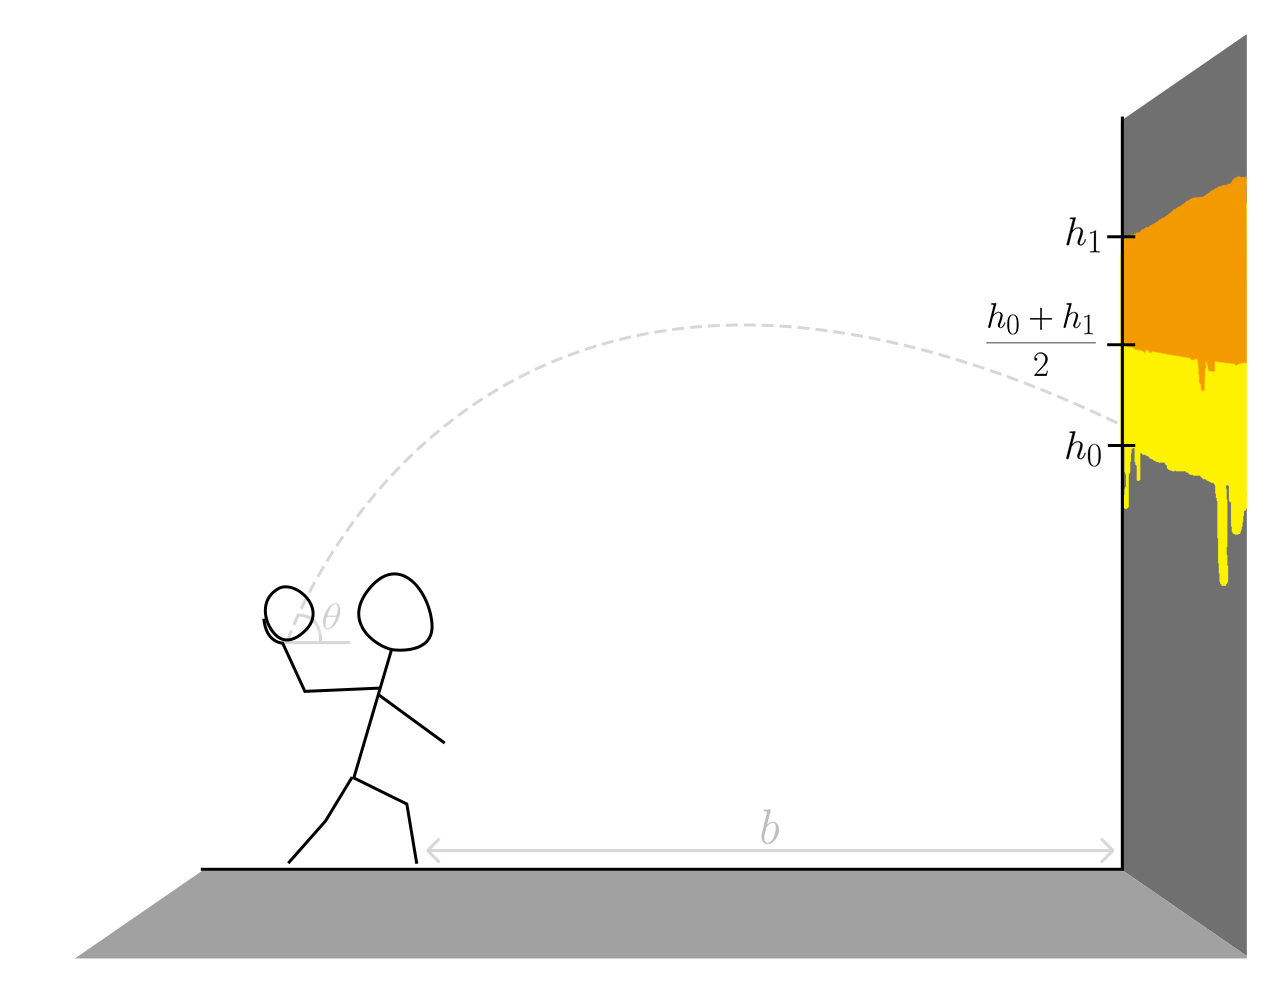
\includegraphics[scale=0.75]{fig_tegning_33-cp1.png}
	\captionof{figure}{Illustrasjon av systemet vi skal basere våres spillsimulering på. }
\end{center}

Ballens høyde over bakken kan modelleres ved
	\begin{align*}
		y(t) &= -\frac{1}{2}g t^2 + v_0t\sin\theta
	\end{align*}
	der $v_0$ er farten personen kaster ballen med, $\theta$ er kastevinkelen og $g = \SI{9.81}{\m.\per \square \second}$. 
	
	\subsection*{a)}
	Skriv en funksjon som returnerer høyden til ballen ved en tid $t$.
	\subsection*{b)}
	Fra modellen kan vi regne oss fram til at ballen vil treffe veggen ved tiden 
	$T = \dfrac{b }{v_0\cos\theta}$, der $b$ er avstanden mellom personen og veggen.
	
	Vi må se på verdien av $y(T)$ for å finne ut hvor mange poeng personen skal få. Antall poeng skal beregnes og returneres fra en funksjon du skal skrive selv. 
	
	Blinken er malt slik at den dekker veggen mellom  høyden $h_0$ og høyden $h_1$ der $h_0 < h_1$. Poengene gis på følgende måte:
	\vspace{.2cm}
	\begin{itemize}
		\item Personen får 0 poeng dersom $y(T) < h_0 \text{ eller } y(T) > h_1$
		\item Personen får 1 poeng dersom $h_0 \leq y(T) <\frac{1}{2}(h_1 + h_0)$
		\item Personen får 2 poeng dersom $\frac{1}{2}(h_1 + h_0) \leq y(T) \leq h_1$
	\end{itemize} 
	\vspace{.2cm}
	
	Skriv et program som skriver ut i en for loop hvor mange poeng personen får ved å kalle på din nyskrevne funksjon dersom $h_0 = 3\,\si{\meter}$, $h_1 = 3.5\,\si{\meter}$, $\theta = \dfrac{\pi}{4}$, $b = 3.5\,\si{\meter}$ for $v_0 = 15,16,19,22\,\si{\meter.\per\second}$. 
	
	
	Filnavn: \texttt{hit\_target.py}
\section*{Oppgave 3.5 - Kast ned stup}
\addcontentsline{toc}{section}{Oppgave 3.5 - Kast ned stup - \texttt{cliff\_throw.py}}
\subsection*{a)}
Vi kaster en ball ned et stup, i en rettlinjet bevegelse med konstant akselerasjon. Vi ignorerer luftmotstand, og regner bare i én dimensjon. Hastigheten til ballen kan beregnes enten som en funksjon av distansen ballen har falt, $x$, eller tiden fra vi kastet den, $t$.
\begin{align}
v &= v_0 + at\\
v &= \sqrt{v_0^2 + 2ax}
\end{align}
(Den nederste er kanskje mer kjent på formen $v^2-v_0^2 = 2ax$).
 
$v_0$ er initialhastigheten ved $t=0$, og $a$ er akselerasjonen, som på jordoverflaten er $a = \SI{9.81}{m/s^2}$. Vi regner positiv retning nedover, slik at posisjon, initialhastigheten og akselerasjonen alle er i positiv retning.
 
Skriv to funksjoner basert på ligningene over, \texttt{velocity1} og \texttt{velocity2}, som returnerer hastigheten fra de tre variablene.
 
Filnavn: \texttt{cliff\_throw.py}
 
 
\subsection*{b)}
Skriv en testfunksjon \texttt{test\_velocity()}, som sjekker om begge hastighetsfunksjonene gir samme hastighet ved et gitt tidspunkt, med samme initialhastighet. Du kan regne distansen ballen har falt ved et gitt tidspunkt fra formelen
\begin{align*}
x = v_0t + \half a t^2
\end{align*}
 
 
\subsection*{c)}
Utvid \texttt{velocity1} fra oppgave a slik at $t$ også kan være en liste av tidspunkter, og funksjonen skal i så fall returnere en liste av hastigheter. Merk at $t$ fortsatt også skal kunne være et tall, og funksjonen skal i så fall returnere en enkelt hastighet, akkurat som før.
 
\textbf{Hint:} Bruk en if-else block til å sjekke typen til $t$, og så en for loop som fyller en liste av hastighets-verdier. Husk at 'et tall' kan være enten en float eller en integer.
 
 
 
 
 
\section*{Oppgave 3.6 - Enda en trekloss}
 \addcontentsline{toc}{section}{Oppgave 3.6 - Enda en trekloss - \texttt{block\_frictions2.py}}
 
Vi ønsker å lage et program som finner ut hvor langt en trekloss med startfart $v_0$ vil komme når den sklir over underlag som består av ulike materialer. Materialet underlaget består av, vil påvirke hvilken friksjonskraft som vil virke på klossen. 
 
Farten og avstanden til klossen ved en tid $t$ kan uttykkes ved:
\begin{align*}
v(t) &= v_0 -  \mu g t \\
x(t) &= v_0t - \frac{1}{2}\mu g t^2
\end{align*}
der $\mu$ er en friksjonskoeffisient og $v_0$ er farten til klossen ved starttiden $t = 0$. 
 
 
\subsection*{a)}
Definér en funksjon som returnerer avstanden $x(t)$ og som tar inn $t, \ v_0 $ og en friksjonskoeffisient $\mu$ som parametre.
\subsection*{b)}
Definér en funksjon som returnerer en liste over hvor langt klossen skled for hver av de ulike friksjonskoeffisienten. 
 
La funksjonen ta inn $\Delta t$ som parameter som er hvor store tidssteg vi ønsker å gjøre pr. tidsmåling av farten til klossen. 
 
Funksjonen skal så bruke en while loop for å finne tiden $t$ når farten $v(t)$ blir mindre eller lik 0. Bruk tiden $t$ som har blitt funnet til å beregne avstanden $x(t)$. Avstanden skal da lagres i en liste. Listen skal så returneres når alle avstandene er ferdig beregnet. 
 
Sett $v_0 = 5\,$m/s, $\Delta t = 0.0001\,$s og listen over friksjonskoeffisienter til å være \texttt{[0.62,0.3,0.45,0.2]}.
\subsection*{c)}
Skriv en testfunksjon som tester om avstandene fra b) er lik den analytiske avstanden $x\qty(\frac{v_0}{\mu g})$ (som er den analytiske tiden hver kloss vil bruke) for hver friksjonskoeffisient $\mu$. En passende grense for å teste om de beregnede avstandene er lik den analytiske avstanden er $10^{-7}$ i denne oppgaven. 
 
Kall tilslutt på testfunksjonen for å sjekke om din implementasjon fra b) stemmer overens med den analytiske avstanden for hver friksjonskoeffisient $\mu$.  
 
Filnavn: \texttt{block\_frictions2.py}
\end{document}
 
 
    
